\documentclass[11pt, oneside]{book}   	% use "amsart" instead of "article" for AMSLaTeX format
\usepackage{geometry}                		% See geometry.pdf to learn the layout options. There are lots.
\geometry{letterpaper}                   		% ... or a4paper or a5paper or ... 
%\geometry{landscape}                		% Activate for rotated page geometry
%\usepackage[parfill]{parskip}    		% Activate to begin paragraphs with an empty line rather than an indent
\usepackage{graphicx}				% Use pdf, png, jpg, or eps§ with pdflatex; use eps in DVI mode
								% TeX will automatically convert eps --> pdf in pdflatex		
\usepackage{amssymb}
\usepackage{amsmath}
\usepackage{mathtools}
\usepackage{tikz}
\usetikzlibrary{shapes.geometric, arrows}

\tikzstyle{data} = [rectangle, rounded corners, minimum width=3cm, minimum height=1cm,text centered, draw=black, fill=red!30]
\tikzstyle{program} = [rectangle, minimum width=3cm, minimum height=1cm, text centered, draw=black, fill=orange!30]
\tikzstyle{database} = [diamond, minimum width=3cm, minimum height=1cm, text centered, draw=black, fill=green!30]
\tikzstyle{arrow} = [thick,->,>=stealth]

%SetFonts

%SetFonts


\title{daPlan}
\author{nd2}
%\date{}							% Activate to display a given date or no date
\begin{document}
\maketitle
\chapter{The General Plan}
\section{Overview and Goals}
The goal is to get that bread by optimizing lineups in daily fantasy games for NBA.\\
\\
The whole process can be broken down into the following : \\
$\bullet$ Data Collection Methods\\
$\bullet$ Data Crunching Methods\\
$\bullet$ The Pipeline \\
\\
I will go over the detail in the following sections, but the ultimate goal and objective is for my to garner some resources for further ventures. To garner resources effectively I must create a automated system that is :\\
\\
$\bullet$ Debuggable : ease of changes to workflow, insertion of new data sources / methods of analysis should be easy\\
$\bullet$ Effective : Strategy should work\\
$\bullet$ Concise : optimization and speed can come later, but documentation should be clear and speed of understanding should be constant\\
\\
\chapter{Data Collection Methods}
The priority of my data collection is to obtain information that will allow me to make better heuristics. I will be storing this data (except media) in a local PSQL database \\
\\
\\
\section{nba.com}
game stats
\section{basketball reference}
coaching
\section{MySportsFeed}
salaries
\section{rotogrinders}
predictions
\section{nbaall.co}
videos
\section{}

Areas to collect data for :\\
$\bullet$ discrete stats\\
$\bullet$ media\\
$\bullet$ player status (injury, depth chart)\\
$\bullet$ projections \\
$\bullet$ player tracking, location data\\
\\

\chapter{The Pipeline}
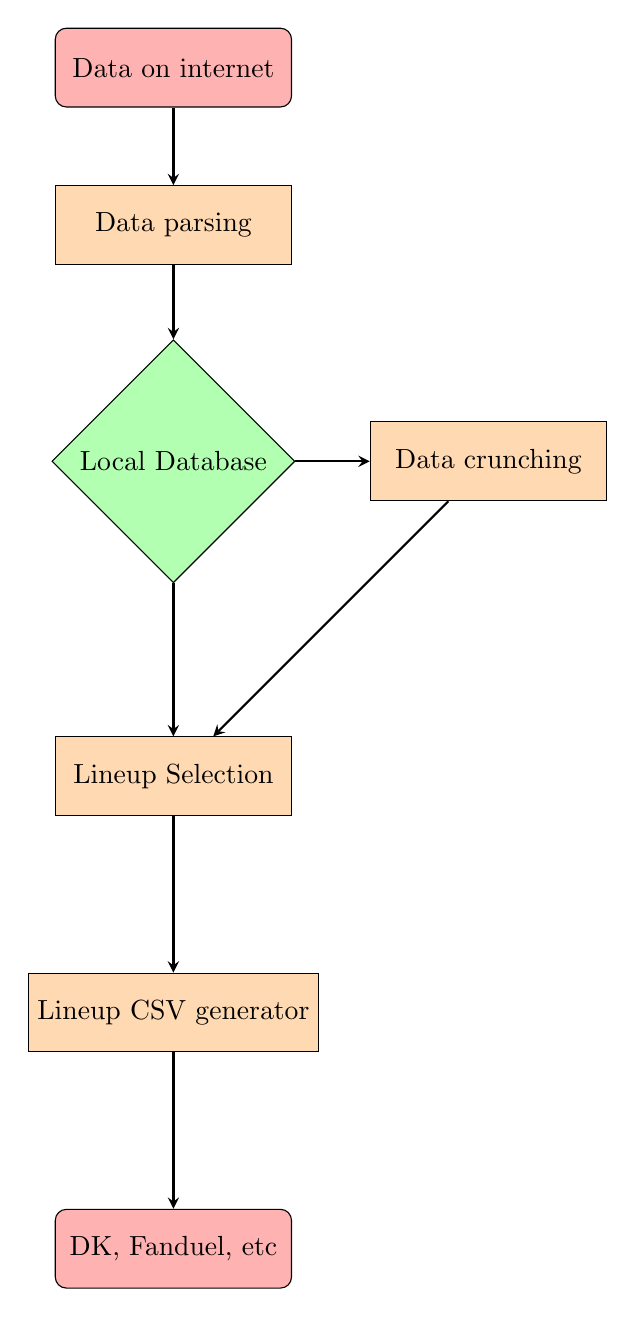
\begin{tikzpicture}[node distance=2cm]
\node (internet) [data] {Data on internet};
\node (web scraper) [program, below of =internet] {Data parsing};
\node (local database) [database, below of=web scraper, yshift=-1cm] {Local Database};
\node (data crunching) [program, right of = local database, xshift=2cm] {Data crunching};
\node (lineup selection) [program, below of=local database, yshift = -2cm] {Lineup Selection};

\node (lineup generator) [program, below of=lineup selection, yshift = -1cm] {Lineup CSV generator};
\node (game website) [data, below of = lineup generator, yshift = -1cm] {DK, Fanduel, etc};

\draw [arrow] (internet) -- (web scraper);
\draw [arrow] (web scraper) -- (local database);
\draw [arrow] (local database) -- (data crunching);
\draw [arrow] (local database) -- (lineup selection);
\draw [arrow] (data crunching) -- (lineup selection);
\draw [arrow] (lineup selection) -- (lineup generator);
\draw [arrow] (lineup generator) -- (game website);


\end{tikzpicture}

\section{lineup generator}
4 stage process: bottom down kinda thing \\
Manually download salary csv file\\
Salary csv parser : will generate multiple lists of lists. Each list of lists corresponds to one "gameset"
\\
(Insert) lineup generator : will be fed the output of csv parser, do additional stuff to this output, convert to np array and perform (insert) on it. Will spitout arrays that contains player's id + position matrix. So  8 X (1 + 8) array's (depending on amount of lineups (insert) decides to do ). \\
Lineup Writer : acts like an overseer to all the lineup(s) generated by each individual lineup generator.  


\section{data crunching}
The spider rg predictions scrapes from rotogrinders their predictios into the psql table rotogrinders predictions. The nba names may not match up, but that will show up when I do the csv parser


\chapter{Sources}
\section{Picking Winners Using Integer Programming}
Paper provides nice solution to optimizing lineups. Main points is on minimizing similarity between different lineups, by constraining covariance with previous lineups. Lineups are picking one by one in greedy way that maximizes objective function while also satisfying variance constraints mentioned above. Player heuristics are also assumed to be normal RV's. An important key when constructing a lineup is to pick players with positive correlations to increase chances such that when they all do well they all do well. Also, reduce pairwise correlation for two lineups A and B, pairwise here is simply the pairing of A's and B's entries. Reason we want potentially negative correlation between lineups is that we want to "cover" more of the possible game space. Increase pairs with negative correlation and decrease pairs with positive correlation. The important constraints used are the lower bound for the variance of a lineup, and upper bound covariance between current lineup I am picking and already picked lineups. 

\chapter{Data Crunchin}
I will be focusing on the quarter jukebox games. My objective is to submit 20 (max per game) entries such that these 20 entries encompass my strategies. \\ First I need to garner some more confidence in my algorithms befor emoving to the one dollar variant of the 20 entries, and so on. Once I get to a certain lvl I can perhaps aim for the max 150 entries games, those require more capitol though. I actually enjoy the 150 games ATM, as I believe more entries = higher chance of winning. In fact, I hereby state that I will not aspire at all to output the best "one", as I believe there is too much variability. What I will aim is to consistently output a good 170 lineups.  
\\
My heursitc methods will output a rating for each player\\
My lineup generation method will use this heurstic and solve an optimization problem that maximizes the sum of this heurstic given the constraints and method-specific additional constraints\\
\\
To analyse the uncertainty, one has to take a top down approach, as the uncertainty trickles down. First a player can play better or worse. A heuristic can either over estimate or underestimate the true FP value of that player. There is uncertainty in the accuracy of the heuristic. As a result the optimization given the heuristic has uncertainty.
\\
why dont I do some convolution correlation stuff.
\\
pertubations of input heuristic, output lineups
\\
Todo:\\
how to introduce more variance in my lineups\\
Run my cruncher's on other machines???

\section{heuristics} 
\subsection{The in house method}
First I need to do some correlation analysis on a day to day basis to see what influences a person's FP. 
\\
Problems:\\
How to get constraint for number of players used max in teams, or number of teams user has to pick from
\subsection{The copycat oracle}
Use rotogrinders predictions, construct lineup that maximizes sum of predicted FP while satisfying constraints. Basically formulate IP following the outline given in Paper and/or some self modifications\\
\\
When grabbing rotogrinders predictions, I run across a couple problems. First each dk csv pertains to only a segment of the games. Rotogrinders scrapes gives me all the players for all the segments. Available segments yet, so in a sense I can trust RG to give me players that I can currently play on. But roto be really wack though\\
\\
The copycat oracle is more oriented towards figuring lineup generation as the heurisitc is already provided in the form of a "black box" courtesy of rotogrinders. The main objective now is to construct lineups in a fashion that alligns with my objectives and biases\\
\\
As of 1/14 the connecting of rg data works, now on to the strategies\\
\subsection{9 life cat}
Using the copycat oracle, tweek the values of each player by adding some noise to the fantasy point values. Perhaps perform a function on the ceiling,floor and expected ot get some other heurstic. Then feed to the lineup generator see how it differs from the one without noise.


\\
Todo\\
Determine the best numbers to use in constraint


\section{lineup generation}


\subsection{the copy cat naive}
naive way involves 17 lineups picked to maximize FP based on player heuristics\\
\subsection{the copy cat n variant}
A generalization of the naive, naive is the 1 variant. Essentially add constraint of the number of different players between lineups.
\subsection{naive + n variant}
The whole point of doing n variant is to increase "variance" of the lineups. When doing naive, the lineups generated could potentially use the same players with a couple swaps. In this strategy, I shall combine the two variants. Running the naive variant will allow me to see the "best" lineups. Using the optimal values from the naive variant as a benchmark, I shall running n variant to output more diverse lineups. Depending on how much predicited optimality I am willing to sacrifice, I will keep a fragment of all these generated lineups.
\\
Let $N$ be the number of unique players used for all lineups \\
Let $n_{a,b,c}$ be the number of unique player used for lineups $a,b$ generated from the $c$ variant\\
Doing a pairwise sum over all $n$'s and then averaging this sum\\
\begin{gather}
\frac{\sum_{c} n_{a,b}}{|c|}, |c| \text{ represents number of lineups generated with c variant}
\end{gather}
\\
\\
\subsection{the build around star}
Generate the "stars" on each team available today. "Stars" are defined to be the top 3(2?) FP predicted players on each team available. Essentially run some variant of the copycat's with additional constraint that this star is used in all lineups.
\subsection{the spread it out}
Naive lineup generation but with stricter constraints on number of players in each team, and number of games. 


\section{lineup writing}
Curently, after running some lineup generator I directly write the outputs to a csv file. I think I should develop an "overlord" type system that takes in all the outputs of eventually the different lineup generators. Take em in, does a little more magic and then spits out the final numbers.
\subsection{The Overseer}
At the moment I am essentially the Overseer. One function of the overseer is to prematurely generate the lineups for different "injury" scenarios. I will have multiple csv files that account for the "absence" of certain players. Eventually the Overseer will enter trivial lineups way ahead of game start to "get spots" (I do not want the contests to fill up). Then as the actual tip off time approaches, Overseer will proceed to actually update those entries' lineups to ones Overseer has pondered over. \\
\\
The main purpose of the Overseer is that it is the final decision maker for what lineups to spit out. It will aggregate all the outputs of the various lineup generators and depending on strategy output the final set of lineups.\\
\\
It will take care of the injury problem. The first layer of injury detection is through rotogrinders. Those that are not on the scraped list will be removed from the gameset.
\\
\subsubsection{Injuries}
I need to know who is not gonna play. The Julius Randle fiasco that was induced from my lack of this shall be remembered. 



\chapter{Todo}
Test my updating and lineup generating sequence, so far so good\\

Start tracking rotogrinders predictions : do this first, tbh I actually dont care about this. Cus imma treat rotogrinders as my black box/oracle, and it really is a black box in some sense\\

Start making lineup upload process more modularized\\

Expand copycat : put some more variation in the lineups?\\

Start thinking about in house analytics : \\
Start thinking aout different strats\\


[URGENT] \\
Solve the time problem, if I were to generate all possible situations I need to have the backups\\
I can constraint the gamesets by time, such that I have all the "scenarios" planned out ahead of time. To swap it is simply a matter of updating the lineup at that time. To update the lineup correctly, I have to account for if the game started or no, 


\chapter{Daily Routine}
dont forget to sudo docker run -p 8050:8050 scrapinghub/splash to allow scrapy to actually scrape\\
\\
$\bullet$ run a base run of db update\\
- when activating the docker for splash, make sure network i am on is the same for when I activated and when I run the spider for rg
$\bullet$ whenever I run something that uses csv parser, I may have to manually alter dk name in players. (dk names need to be change). If using copy cat need to change rg name in players.\\

Setup script
cd Documents/Creations/StudentOfTheGame && source ENV/bin/activate 

sudo docker run -p 8050:8050 scrapinghub/splash
psql basketball
\end{document}
